\begin{lstlisting}
p13 1(2)(3) 4 7 9(2) 11 14 
\end{lstlisting}
\begin{exercise}
\begin{figure}[H]
\centering
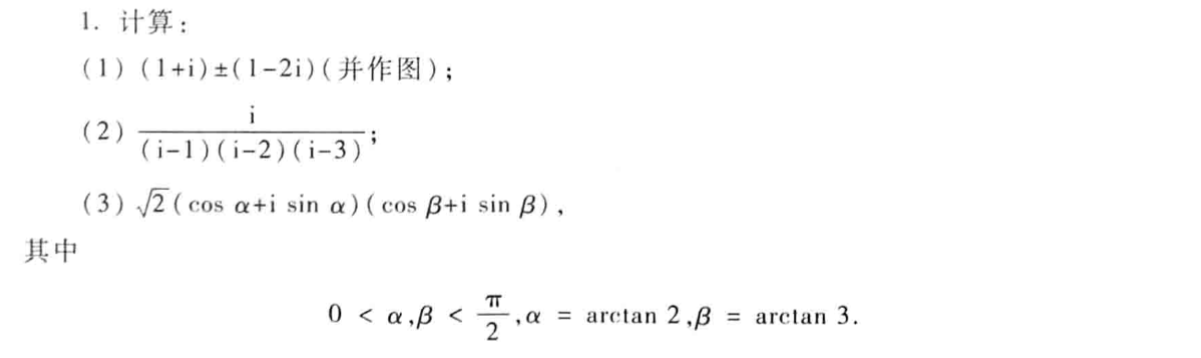
\includegraphics[width=\textwidth]{hw1-20250303.png}
% \caption{}
\label{}
\end{figure}
\end{exercise}
\[
\frac{i}{(i-1)(i-2)(i-3)}=\frac{i(i+1)(i+2)(i+3)}{(-2)(-5)(-10)}= \frac{1}{10}
\]
\[
\sqrt{ 2 }(\cos\alpha+i\sin\alpha)(\cos\beta+i\sin\beta)=\sqrt{ 2 }\left( \frac{1}{\sqrt{ 5 }} +i \frac{2}{\sqrt{ 5 }}  \right)\left( \frac{1}{\sqrt{ 10 }} +i \frac{3}{\sqrt{ 10 }}  \right)=-1+i 
\]
\begin{exercise}
\begin{figure}[H]
\centering
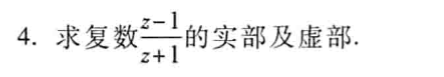
\includegraphics[width=\textwidth]{1-hw1-20250303.png}
% \caption{}
\label{}
\end{figure}
\end{exercise}
$z\coloneqq a+ib$, then
\[
\frac{z-1}{z+1}=\frac{a-1+ib}{a+1+ib}=\frac{(a-1+ib)(a+1-ib)}{(a+1)^{2}-b^{2}}=\frac{a^{2}-(1-ib)^{2}}{a^{2}-b^{2}+2a+1}=\frac{a^{2}+b^{2}+2ib-1}{a^{2}-b^{2}+2a+1}
\]
Hence
\[
\mathrm{Re}\left( \frac{z-1}{z+1} \right)=\frac{\mathrm{Re}(z)^{2}+\mathrm{Im}(z)^{2}-1}{\mathrm{Re}(z)^{2}-\mathrm{Im}(z)^{2}+2\mathrm{Re}(a)+1}
\]
\[
\mathrm{Im}\left( \frac{z-1}{z+1} \right)=\frac{2\mathrm{Im}(z)}{\mathrm{Re}(z)^{2}-\mathrm{Im}(z)^{2}+2\mathrm{Re}(a)+1}
\]
\begin{exercise}
\begin{figure}[H]
\centering
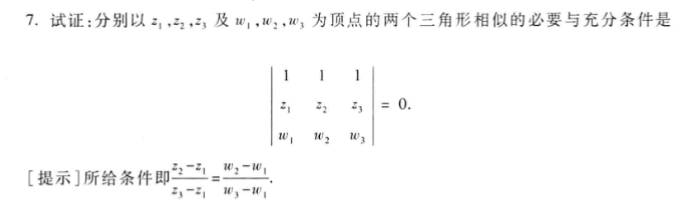
\includegraphics[width=\textwidth]{3-hw1-20250303.png}
% \caption{}
\label{}
\end{figure}
\end{exercise}
Let $Z(\mathrm{Re}(z),\mathrm{Im}(z))$, then
\[
\frac{z_{2}-z_{1}}{z_{3}-z_{1}}=\frac{w_{2}-w_{1}}{w_{3}-w_{1}}\iff\frac{\lvert Z_{1}Z_{2} \rvert }{\lvert Z_1Z_{3} \rvert }=\frac{\lvert W_{1}W_{2} \rvert }{\lvert W_{1}W_{3} \rvert }\text{ and }\angle Z_{2}Z_{1}Z_{3}=\angle W_{2}W_{1}W_{3}\iff \Delta Z_{1}Z_{2}Z_{3}\sim \Delta W_{1}W_{2}W_{3}
\]
\begin{exercise}
\begin{figure}[H]
\centering
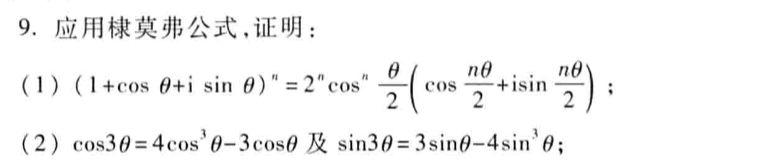
\includegraphics[width=\textwidth]{6-hw1-20250303.png}
% \caption{}
\label{}
\end{figure}
\end{exercise}
\begin{definition}[棣莫弗公式]
\begin{figure}[H]
\centering

\includegraphics[width=\textwidth]{10-hw1-20250303.png}
% \caption{}
\label{}
\end{figure}
\end{definition}
\[
\cos(3\theta)+i\sin(3\theta)=e^{ 3i\theta }=(\cos\theta+i\sin\theta)^{3}=(4\cos ^{3}\theta-3\cos\theta)+i(3\sin\theta-4\sin ^{3}\theta)
\]
\begin{exercise}
\begin{figure}[H]
\centering
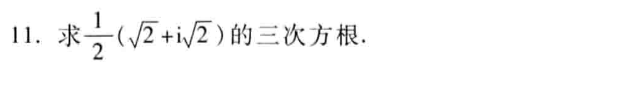
\includegraphics[width=\textwidth]{7-hw1-20250303.png}
% \caption{}
\label{}
\end{figure}
\end{exercise}
Solve the equation:
\[
z^{3}=\frac{1}{2}(\sqrt{ 2 }+i\sqrt{ 2 })=e^{ i\pi/4 }=e^{ i\cdot9\pi/4 }=e^{ i\cdot17\pi/4 }
\]
Then
\[
z_{1}=e^{ i\pi/12 },z_{2}=e^{ i\cdot3\pi/4 },z_{3}=e^{ i\cdot17\pi/12 }
\]
\begin{exercise}
\begin{figure}[H]
\centering
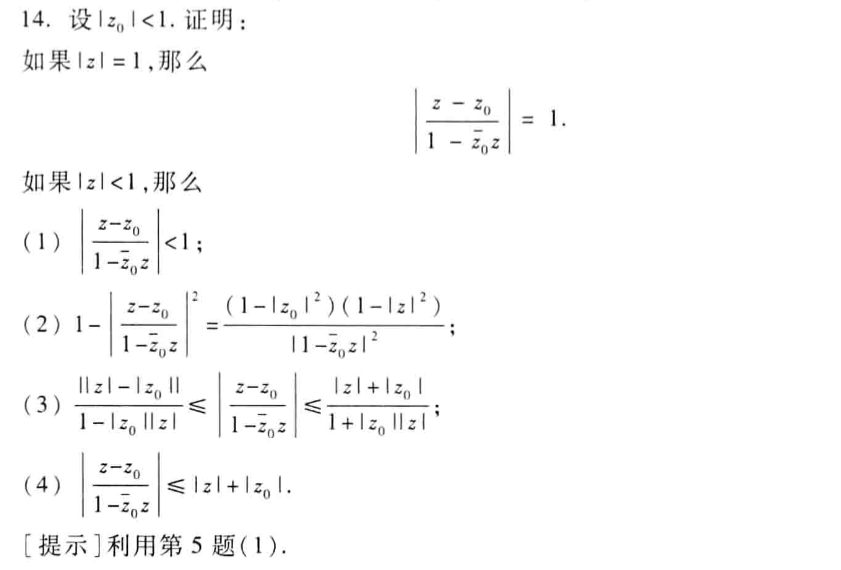
\includegraphics[width=\textwidth]{8-hw1-20250303.png}
% \caption{}
\label{}
\end{figure}
\end{exercise}
\begin{note}
\begin{figure}[H]
\centering
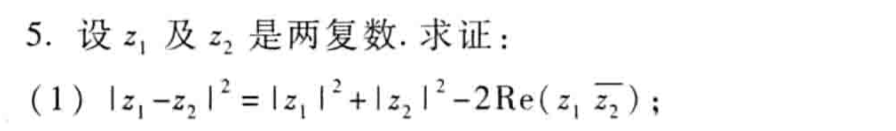
\includegraphics[width=\textwidth]{11-hw1-20250303.png}
% \caption{}
\label{}
\end{figure}
\end{note}
If $\lvert z \rvert=1$, then
\[
\lvert 1-\overline{z_{0}}z \rvert =\lvert 1-\mathrm{Re}(\overline{z_{0}}z)-i\cdot \mathrm{Im}(\overline{z_{0}}z) \rvert =\sqrt{ 1+\lvert \overline{z_{0}}z \rvert ^{2} -2\mathrm{Re}(\overline{z_{0}}z) }=\sqrt{ 1+\lvert z_{0} \rvert ^{2} -2\mathrm{Re}(\overline{z_{0}}z) }
\]
On the other hand
\[
\lvert z-\overline{z_{0}} \rvert =\sqrt{ 1+\lvert z_{0} \rvert ^{2}-2\mathrm{Re}(\overline{z_{0}}z) }
\]
Therefore
\[
\left\lvert  \frac{z-\overline{z_{0}}}{1-\overline{z_{0}}z}  \right\rvert =1
\]
If $\lvert z \rvert<1$, we have $(\lvert z \rvert ^{2}-1)(\lvert z_{0} \rvert ^{2}-1)>0\Rightarrow1+\lvert z \rvert ^{2}\lvert z_{0} \rvert ^{2}>\lvert z \rvert ^{2}+\lvert z_{0} \rvert ^{2}$ then
\[
\left\lvert  \frac{z-z_{0}}{1-\overline{z_{0}}z}  \right\rvert =\frac{\sqrt{ \lvert z \rvert ^{2}+\lvert z_{0} \rvert ^{2}-2\mathrm{Re}(\overline{z_{0}}z) }}{\sqrt{ 1+\lvert z_{0} \rvert ^{2}\lvert z \rvert ^{2}-2\mathrm{Re}(\overline{z_{0}}z) }}<1
\]
And
\[
1-\left\lvert  \frac{z-z_{0}}{1-\overline{z_{0}}z}  \right\rvert ^{2}=\frac{1+\lvert z_{0} \rvert ^{2}\lvert z \rvert ^{2}-\lvert z \rvert ^{2}-\lvert z_{0} \rvert ^{2} }{1+\lvert z_{0} \rvert ^{2}\lvert z \rvert ^{2}-2\mathrm{Re}(\overline{z_{0}}z)}=\frac{\left(1-\left|z_0\right|^2\right)\left(1-|z|^2\right)}{\left|1-\bar{z}_0 z\right|^2}
\]
We have
\[
\left( \frac{\lvert \lvert z \rvert -\lvert z_{0} \rvert  \rvert }{1-\lvert z_{0} \rvert \lvert z \rvert } \right)^{2}=\frac{\lvert z \rvert ^{2}+\lvert z_{0} \rvert ^{2}-2\lvert \overline{z_{0}} \rvert \lvert z \rvert }{1+\lvert z_{0} \rvert ^{2}\lvert z \rvert ^{2}-2\lvert z_{0} \rvert \lvert z \rvert },\qquad \left( \frac{\lvert z \rvert +\lvert z_{0} \rvert }{1+\lvert z_{0} \rvert \lvert z \rvert } \right)^{2}=\frac{\lvert z \rvert ^{2}+\lvert z_{0} \rvert ^{2}+2\lvert \overline{z_{0}} \rvert \lvert z \rvert }{1+\lvert z_{0} \rvert ^{2}\lvert z \rvert ^{2}+2\lvert z_{0} \rvert \lvert z \rvert }
\]
Consider the function
\[
f(x)=\frac{\lvert z \rvert ^{2}+\lvert z_{0} \rvert ^{2}-x}{1+\lvert z_{0} \rvert ^{2}\lvert z \rvert ^{2}-x}=1-\frac{(1-\lvert z \rvert ^{2})(1-\lvert z_{0} \rvert ^{2})}{1+\lvert z_{0} \rvert ^{2}\lvert z \rvert ^{2}-x}
\]
which is decreasing in $(-\infty,1+\lvert z_{0} \rvert ^{2}\lvert z \rvert ^{2})$. Since $-2\lvert \overline{z_{0}} \rvert \lvert z \rvert\leq 2\mathrm{Re}(\overline{z_{0}}z)\leq 2\lvert \overline{z_{0}} \rvert \lvert z \rvert<1+\lvert z_{0} \rvert ^{2}\lvert z \rvert ^{2}$, we have $f(-2\lvert \overline{z_{0}} \rvert \lvert z \rvert)\geq f(2\mathrm{Re}(\overline{z_{0}}z))\geq f(2\lvert \overline{z_{0}} \rvert \lvert z \rvert)$, that is
\[
\frac{\left\|z|-| z_0\right\|}{1-\left|z_0 \| z\right|} \leqslant\left|\frac{z-z_0}{1-\bar{z}_0 z}\right| \leqslant \frac{|z|+\left|z_0\right|}{1+\left|z_0\right||z|}
\]
Therefore,
\[
\left\lvert  \frac{z-z_{0}}{1-\overline{z_{0}}z}  \right\rvert \leq \frac{\lvert z \rvert +\lvert z_{0} \rvert }{1+\lvert z_{0} \rvert \lvert z \rvert }\leq \lvert z \rvert +\lvert z_{0} \rvert
\]